\section{Results}\label{sec:results}

\subsection{The refinement on the lattice task}

\begin{table}[t]
\centering\small
\caption{The device-aware refinement on the $10\times10$ lattice task, scored on the device. Medians over \nSeedsOne{} seeds for the crosstalk device and \nSeedsOneFull{} for the full device; $\sigma$ is the relative standard deviation of the trap intensities in percent and $e$ the efficiency. Rows marked n/a have no entry for that device or metric.}
\label{tab:b1}
\begin{tabular}{@{}l r r r@{}}
\toprule
Method & $\sigma$ on the crosstalk device & $\sigma$ on the full device & $e$ (crosstalk device)\\
\midrule
GS, 30 iterations & \sigmaMfour & n/a & n/a\\
Weighted GS, 30 iterations & \sigmaMsix & n/a & n/a\\
Phase-fixed WGS, 30 iterations & \sigmaMsevenThirty & \sigmaMsevenFull & \effMseven\\
Phase-fixed WGS, 100 iterations & \sigmaMsevenHundred & n/a & n/a\\
Refinement without the device model & \sigmaNoModel & \sigmaNoModelFull & n/a\\
Device-aware refinement & \sigmaBOne & \sigmaBOneFull & \effBOne\\
\bottomrule
\end{tabular}
\end{table}

Table~\ref{tab:b1} and Fig.~\ref{fig:b1} give the main comparison. On the crosstalk device, phase-fixed WGS leaves a spread of \sigmaMsevenThirty{} percent at 30 iterations and \sigmaMsevenHundred{} percent at 100, although it reaches \sigmaMsevenIdeal{} percent on the ideal model: the crosstalk costs a factor of about \costXtalk{}, as Proposition~\ref{prop:floor} anticipates, and the baseline at
100 iterations is no better than at 30, which excludes more iterations as the explanation of any gain. The refinement reduces the spread to a median of \sigmaBOne{} percent (mean \sigmaOneMean{} with a standard deviation of \sigmaOneSd{} over the seeds, largest value \sigmaBOneMax{} percent). Against the better of the two baseline runs the factor of Eq.~\ref{eq:factor} has a geometric mean of \ratioOneGm{} with a 95 percent interval of \ratioOneCiLo{} to \ratioOneCiHi{}, a median of \ratioOneMed{} and a range of \ratioOneMin{} to \ratioOneMax{}, and the
efficiency ratio has a median of \effRatioOne{} with a smallest value of \effRatioOneMin{}. H1 therefore holds on every seed with a wide margin on the factor and a narrow one on the efficiency: the loss of efficiency is about half a percent against the allowed ten. The factor varies from seed to seed with the baseline's own spread, so the distribution and not one seed is the result (Fig.~\ref{fig:b1}b).

The control that keeps the structure of the refinement and removes the device model from the loop stays at \sigmaNoModel{} percent, the level of the baseline, so H2 holds: the gain comes from the device model and not from the extra iterations or from the gradient steps. The refinement pays for this on the ideal model: scored without the device its spread is \sigmaBOneIdeal{} percent, because its hologram is built to cancel the crosstalk and not to be uniform before it. Figure~\ref{fig:b1tradeoff}
shows the same result as a trade-off: the baselines and the control sit together at a spread of several percent, the refinement sits two orders of magnitude lower at the same efficiency, and no point of the refinement buys its uniformity with light. The curve of Fig.~\ref{fig:b1model}b shows how the refinement gets there on seed 1: the spread falls during the outer iterations and the returned iterate is the last or one of its tail.

\begin{figure}[t]
\centering
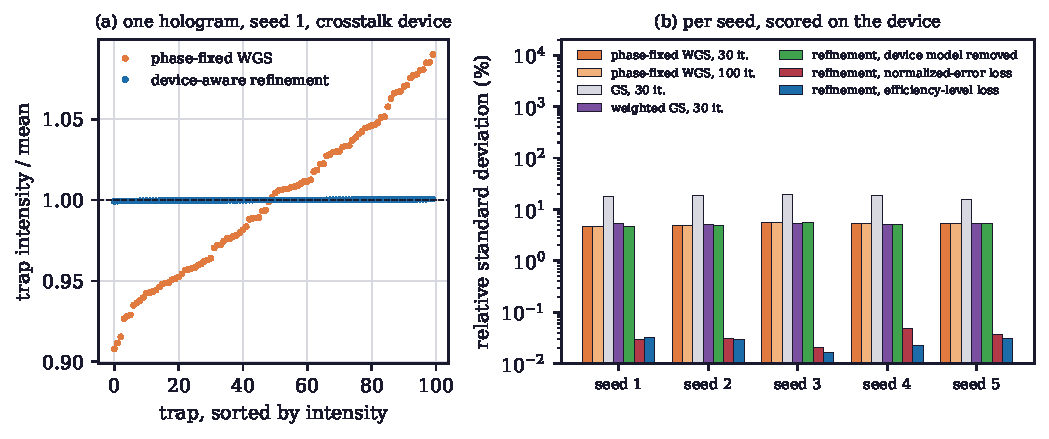
\includegraphics[width=\textwidth]{fig-b1.pdf}
\caption{The device-aware refinement on the crosstalk device. (a) Sorted trap intensities of one hologram (seed 1): phase-fixed WGS leaves a spread, the refinement is flat. (b) Relative standard deviation on the device for every seed on a logarithmic scale: the baselines, the refinement with the device model removed from the loop, the refinement with the efficiency-level loss and the refinement with the normalized-error loss of Schroff et al.}
\label{fig:b1}
\end{figure}

\begin{figure}[t]
\centering
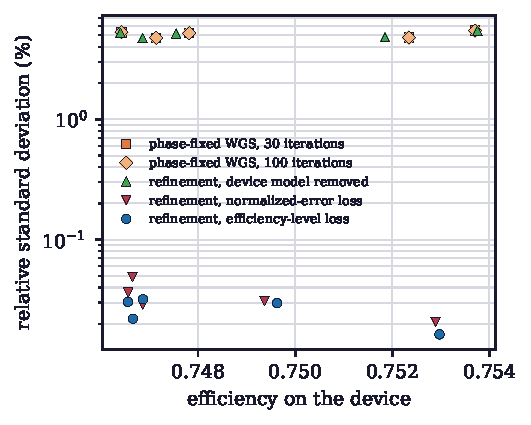
\includegraphics[width=0.5\textwidth]{fig-b1-tradeoff.pdf}
\caption{Efficiency against relative standard deviation on the crosstalk device, one marker per seed: phase-fixed WGS at 30 and 100 iterations, the refinement with the device model removed from the loop, the refinement with the efficiency-level loss and the refinement with the normalized-error loss. The vertical axis is logarithmic.}
\label{fig:b1tradeoff}
\end{figure}

\begin{figure}[t]
\centering
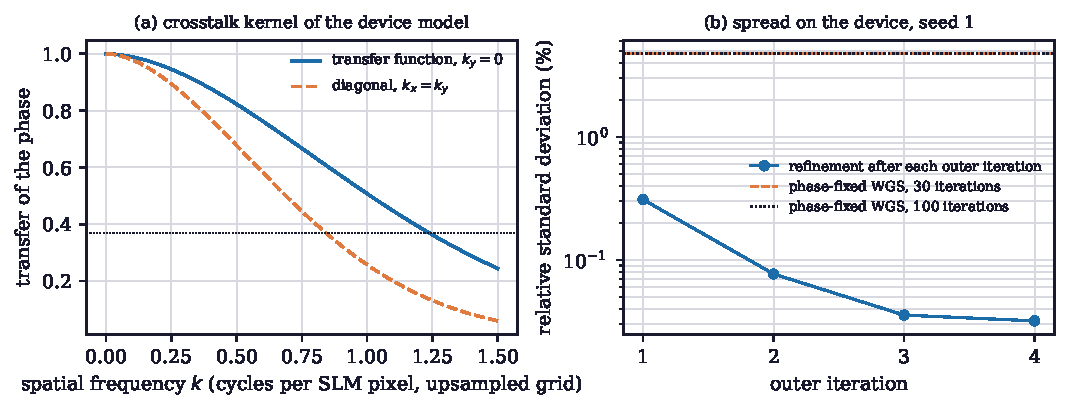
\includegraphics[width=\textwidth]{fig-b1-model.pdf}
\caption{Device model and convergence of the refinement. (a) Transfer function of the crosstalk kernel of Eq.~\ref{eq:kernel} along one axis and along the diagonal, in cycles per SLM pixel on the upsampled grid, the unit that the engine gives the source's inverse pixels. (b) Relative standard deviation of the refinement after each outer iteration on seed 1 against the two baseline levels.}
\label{fig:b1model}
\end{figure}

\subsection{The normalized-error loss of Schroff et al.}

\begin{table}[t]
\centering\small
\caption{The efficiency-level loss of the refinement against the normalized-error loss of Schroff et al., both through the same warm start, device model, conjugate-gradient optimizer and safeguard, on the lattice task: $n$ seeds, median and range of the spread $\sigma$, geometric-mean factor over phase-fixed WGS with its 95 percent interval, median efficiency ratio and median seconds per hologram.}
\label{tab:schroff}
\resizebox{\textwidth}{!}{\begin{tabular}{@{}l l r r r r r@{}}
\toprule
Task & Method & $n$ & $\sigma$ median (range) (\%) & Factor over phase-fixed WGS, 95\% interval & $e$ ratio & Seconds per hologram \\
\midrule
crosstalk device & device-aware refinement (default) & 5 & 0.030 (0.016 to 0.032) & 201.3 (132.9 to 304.9) & 0.999 & 34 \\
crosstalk device & normalized-error loss of Schroff et al. & 5 & 0.031 (0.021 to 0.049) & 159.9 (107.0 to 239.1) & 0.999 & 34 \\
4-bit device & device-aware refinement (default) & 5 & 0.242 (0.202 to 0.335) & 23.5 (18.6 to 29.6) & 0.997 & 59 \\
4-bit device & normalized-error loss of Schroff et al. & 5 & 0.222 (0.172 to 0.258) & 26.1 (20.2 to 33.9) & 0.997 & 58 \\
\bottomrule
\end{tabular}
}
\end{table}

Table~\ref{tab:schroff} and Fig.~\ref{fig:schroff} run the closest published loss through the same optimizer. On the crosstalk device the normalized-error loss reaches a median spread of \schroffXSig{} percent (range \schroffXSigMin{} to \schroffXSigMax{}) against \ablBFullSig{} percent for the efficiency-level loss (range \ablBFullSigMin{} to \ablBFullSigMax{}), a factor over phase-fixed WGS of \schroffXFac{} (interval \schroffXFacLo{} to \schroffXFacHi{}) against \ratioOneGm{} (interval \ratioOneCiLo{} to \ratioOneCiHi{}), at the same efficiency ratio (\schroffXEffRatio{}, smallest \schroffXEffRatioMin{}) and the same median time per hologram, \schroffXSeconds{} s. The efficiency-level loss has the lower spread on \schroffXDefaultBeats{} of the \schroffXN{} seeds and the normalized-error loss on \schroffXBeatsDefault{}; the medians differ by a ratio of \schroffXRatio{} and the ranges overlap. On the full device the normalized-error loss reaches \schroffFSig{} percent (range \schroffFSigMin{} to \schroffFSigMax{}) against \ablBFFullSig{} percent (range \ablBFFullSigMin{} to \ablBFFullSigMax{}), a factor of \schroffFFac{} (interval \schroffFFacLo{} to \schroffFFacHi{}) against \ratioOneFullGm{} (interval \ratioOneFullCiLo{} to \ratioOneFullCiHi{}); here the normalized-error loss has the lower median, the lower spread on \schroffFBeatsDefault{} of \schroffFN{} seeds, and a ratio of the two medians of \schroffFRatio{}, at an efficiency ratio of \schroffFEffRatio{} and \schroffFSeconds{} s against \secBFMedian{} s. The two losses are indistinguishable at these seeds. H5 holds on both devices: the median of the efficiency-level loss lies inside the range of the normalized-error loss, \ablBFullSig{} inside \schroffXSigMin{} to \schroffXSigMax{} and \ablBFFullSig{} inside \schroffFSigMin{} to \schroffFSigMax{}. Where the normalized-error loss is lower, on the full device, the paper reports it as lower, and the abstract and the discussion say so.

\begin{figure}[t]
\centering
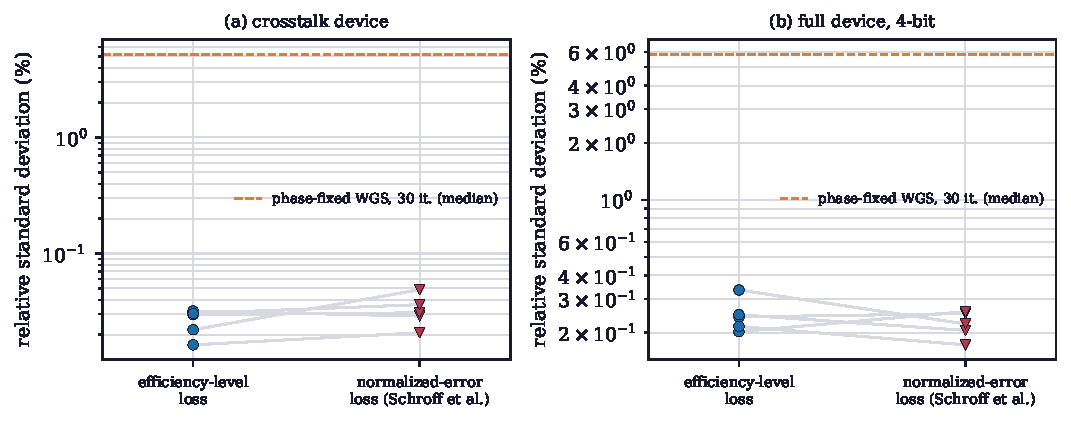
\includegraphics[width=\textwidth]{fig-schroff.pdf}
\caption{Spread per seed of the efficiency-level loss and of the normalized-error loss of Schroff et al.\ through the same optimizer. (a) Crosstalk device, $10\times10$ lattice. (b) Full device with a 4-bit quantizer. Lines join the two runs of one seed; the vertical axes are logarithmic and the horizontal line is the median of phase-fixed WGS at 30 iterations.}
\label{fig:schroff}
\end{figure}

Proposition~\ref{prop:losses} reads this result. For equal traps and the default steepness the two losses are the same function at the point where an outer iteration sets its target, and their gradients differ by a push along the gradient of the total light whose weight is the loss itself. Both start from the same warm start, so the first descent direction differs by that small term, and the spreads that the two losses reach differ by less than the spread between seeds. The loss is therefore not where the gain of the method comes from. What carries the gain is the device model in the loop and the conjugate-gradient steps through it (Section~\ref{sec:ablation}), which both losses share.

\subsection{Full device and the small grid of the studio}

With a \parBits{}-bit quantizer and a fill factor of \parFill{} added, the baseline spread is \sigmaMsevenFull{} percent and the refinement reaches \sigmaBOneFull{} percent (mean \sigmaOneFullMean{}, standard deviation \sigmaOneFullSd{}, over \nSeedsOneFull{} seeds). The geometric-mean factor is \ratioOneFullGm{} with a 95 percent interval of \ratioOneFullCiLo{} to \ratioOneFullCiHi{} (median \ratioOneFullMed{}, range \ratioOneFullMin{} to \ratioOneFullMax{}) at \effRatioOneFull{} of the efficiency, and the model-free control stays at
\sigmaNoModelFull{} percent. The factor is lower than on the crosstalk device because the quantizer is differentiated as the identity; it is still above two on every seed, so H1 holds on this device as well.

The small $8\times8$ array on a $\bakeCeightPix^2$-pixel SLM, with \parBits{}-bit phase, crosstalk, a fill factor of \parFill{}, \bakeCeightFlicker{} rad of flicker and a fixed budget of \bakeCeightIters{} iterations, is the device-limited case of the studio. Its committed scores are \bakeCeightBOneSigma{} percent for the refinement and \bakeCeightMsevenSigma{} percent for phase-fixed WGS on the bake's seed, a factor of \bakeCeightRatio{} at an efficiency ratio of \bakeCeightEffRatio{}; over the \bakeCeightSeedsN{}
seeds of the committed ranges the factors are \bakeCeightSeedRatios{}, of which \bakeCeightSeedsTwo{} is two or more, and the ratio of the means is \bakeCeightRatioThree{}. The factor is not a constant: it depends on the grid, the device, the budget and the seed. The benefit shrinks as the device departs from what the optimizer models, since flicker is scored and not modelled and the quantizer is only straight-through.

\subsection{The geometries of the benchmark}

Table~\ref{tab:bench} and Fig.~\ref{fig:bench} repeat the comparison on the geometries of the studio's benchmark, on the device with flicker. At \benchOneBudget{} iterations with the default parameters the median factor over the \benchOneDevN{} geometries is \benchOneDevMed{} (range \benchOneDevMin{} to \benchOneDevMax{}) at a median efficiency ratio of \benchOneDevEff{}, and \benchOneDevPass{} of them meet both thresholds: the ring, the random set and the two large sets. The factors are \benchOneDevList{}. These cells hold \benchOneDevSeeds{} seeds for the refinement, so by the win rule none of them is a win; they are ranges. H3 is refuted by the square lattice, whose factor is below two, although the large lattice meets both thresholds. On the quasi-periodic set the refinement leaves the spread at the level of the baseline (the factor is near one, with overlapping interquartile ranges).

\begin{table}[t]
\centering\small
\caption{The refinement against phase-fixed WGS on the geometries of the studio's benchmark, on the device with flicker. The spreads are medians over the seeds of each cell at \benchOneBudget{} iterations with the interquartile range in parentheses; the first $n$ column gives the seeds of the refinement and of phase-fixed WGS at that budget. The factor is the ratio of the median spreads and the efficiency ratio the ratio of the median efficiencies; $t$ is the median seconds per hologram on the device at that budget. The equal-time reading applies the win rule to the rows at the wall-clock budget of the second $n$ column, with its seeds, and the last column states whether both thresholds of H1 are met at \benchOneBudget{} iterations.}
\label{tab:bench}
\resizebox{\textwidth}{!}{\begin{tabular}{@{}l r r r r r r r r r l l@{}}
\toprule
Geometry & Traps & $n$ & \shortstack[r]{$\sigma$ phase-fixed\\WGS (\%)} & \shortstack[r]{$\sigma$ refinement\\(\%)} & Factor & $e$ ratio & \shortstack[r]{$t$ phase-fixed\\WGS (s)} & \shortstack[r]{$t$ refinement\\(s)} & $n$ at 1~s & \shortstack[l]{Reading at\\equal time} & \shortstack[l]{Both\\thresholds} \\
\midrule
G1 Square 10 x 10 & 100 & 2, 20 & 26.44 (25.09 to 27.55) & 13.91 (13.77 to 14.05) & 1.90 & 0.952 & 2.73 & 779 & 5, 20 & proposed & no \\
G2 Ring of 36 traps & 36 & 2, 20 & 16.96 (16.12 to 17.94) & 8.31 (8.02 to 8.61) & 2.04 & 0.981 & 0.367 & 810 & 5, 20 & proposed & yes \\
G3 Random 100 traps & 100 & 2, 20 & 20.67 (20.24 to 20.83) & 4.28 (4.28 to 4.29) & 4.82 & 0.958 & 0.616 & 822 & 5, 20 & proposed & yes \\
G4 Quasi-periodic 119 & 119 & 2, 20 & 85.16 (63.96 to 117.28) & 81.09 (73.26 to 88.92) & 1.05 & 0.996 & 0.724 & 832 & 5, 20 & tie & no \\
G6a Large lattice 32 x 32 & 1024 & 2, 6 & 30.06 (29.76 to 30.39) & 13.99 (13.96 to 14.01) & 2.15 & 0.923 & 7.44 & 1939 & 5, 6 & tie & yes \\
G6b Disordered 819 & 819 & 2, 7 & 9.16 (8.88 to 9.26) & 4.39 (4.39 to 4.40) & 2.08 & 0.992 & 5.41 & 1940 & 5, 7 & tie & yes \\
\bottomrule
\end{tabular}
}
\end{table}

\begin{figure}[t]
\centering
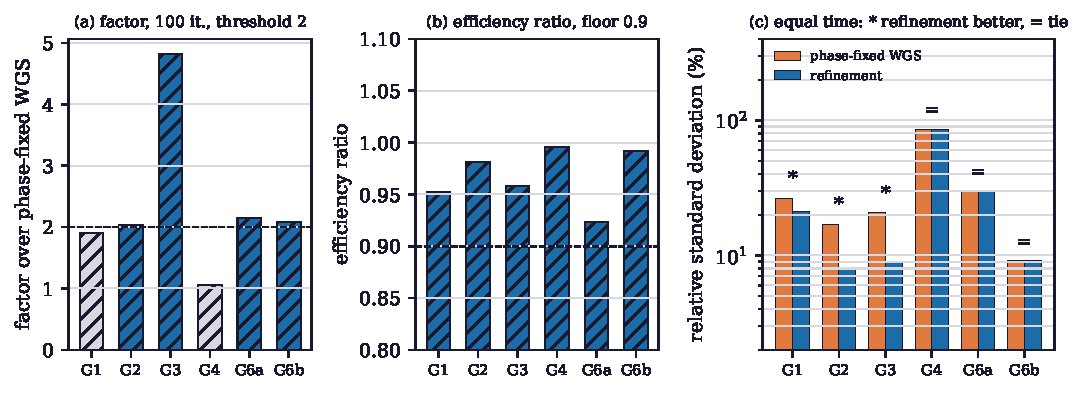
\includegraphics[width=\textwidth]{fig-bench.pdf}
\caption{The refinement on the benchmark geometries of the device with flicker. (a) Factor of the spread over phase-fixed WGS at \benchOneBudget{} iterations with the threshold of two; hatched bars are cells of two seeds, read as ranges. (b) Ratio of the efficiencies with the floor of $0.9$. (c) Relative standard deviation at the equal wall-clock time of the benchmark, median over the seeds of each side; the marker shape gives the reading of the win rule.}
\label{fig:bench}
\end{figure}

The equal-time rows give the reading that the win rule allows. At the time budget of \benchOneTimeBudget{} s per hologram, with \benchOneWinMinSeeds{} seeds or more on each side, the refinement is read as better than phase-fixed WGS on \benchOneDevTimeProposed{} of the \benchOneDevCells{} geometries (the square lattice, the ring and the random set) and ties on \benchOneDevTimeTie{} (the quasi-periodic set and the two large sets), with the interquartile ranges overlapping in each tie, and phase-fixed WGS wins on none (\benchOneDevTimePublished{}). The medians at that budget are, for the refinement against phase-fixed WGS, \benchTimeSigRefGeoOne{} against \benchTimeSigMsevenGeoOne{} percent on the square lattice, \benchTimeSigRefGeoTwo{} against \benchTimeSigMsevenGeoTwo{} on the ring and \benchTimeSigRefGeoThree{} against \benchTimeSigMsevenGeoThree{} on the random set. H4 is therefore refuted: the refinement does not read as better on every geometry. On the ideal device of the same benchmark, the same rule reads \benchOneIdealTimeProposed{} geometry as better for the refinement, \benchOneIdealTimePublished{} as better for phase-fixed WGS and \benchOneIdealTimeTie{} as ties, over \benchOneIdealCells{} geometries, so the equal-time advantage belongs to the device rows and is not general. Within the one-second rows the refinement does little conjugate-gradient work: its median iterations, which count the \parWarm{} warm-start iterations plus the accepted steps, are \benchOneSecItersMin{} to \benchOneSecItersMax{} over the six geometries, so the equal-time reading compares a nearly unrefined hologram with the baseline, and the deadline overruns the budget by \benchOneSecOverrunMin{} to \benchOneSecOverrunMax{} s in the median (at most one evaluation of the device model, as the engine allows).

\subsection{Cost in time on the device}

The time per hologram is the price of these results. On the acceptance task of the crosstalk device the refinement takes a median of \secBXMedian{} s, against \secMsevenThirty{} s for phase-fixed WGS at 30 iterations and \secMXSevenHundred{} s at 100 (plain GS \secMfourThirty{} s, weighted GS \secMsixThirty{} s), a ratio of \timeRatioX{} to the 100-iteration baseline; on the full device the median is \secBFMedian{} s against \secMFSevenHundred{} s, a ratio of \timeRatioF{}. On the geometries of the benchmark at \benchOneBudget{} iterations the refinement takes \benchHundredSecRefMin{} to \benchHundredSecRefMax{} s per hologram against \benchHundredSecMsevenMin{} to \benchHundredSecMsevenMax{} s for phase-fixed WGS. The long budget is not where the quality is made. At 10, 30 and 100 outer iterations the median spread of the refinement is identical to the precision of the benchmark file in \benchBudgetSameCells{} of \benchBudgetCells{} geometries, while the time grows with the budget; on the square lattice the accepted work stays at \benchGOneIters{} iterations (the warm start plus the accepted conjugate-gradient steps) whereas the evaluations of the device model grow from \benchGOneEvalTen{} at 10 outer iterations to \benchGOneEvalHundred{} at 100, and the time from \benchGOneSecTen{} s to \benchGOneSecHundred{} s. The time per hologram at a long budget is therefore an upper bound set by the loop, which keeps evaluating the device model, and not by the accepted work, which stays at \benchGOneIters{} iterations while the evaluations grow from \benchGOneEvalTen{} to \benchGOneEvalHundred{}. The cost at the budget where the spread stops changing, 10 outer iterations, is \benchTenSecRefMin{} to \benchTenSecRefMax{} s per hologram on the six geometries against \benchTenSecMsevenMin{} to \benchTenSecMsevenMax{} s for phase-fixed WGS. A hologram that the experiment needs in seconds is therefore out of the reach of the refinement; one that is computed offline and displayed many times is not. The times are wall-clock seconds of a CPU run on a machine that other jobs also loaded, so they are read as orders of magnitude, seconds against minutes, and not as precise ratios.

\subsection{Outcome of each hypothesis}

Table~\ref{tab:outcome} summarizes the outcome of the hypotheses of Section~\ref{sec:design} with the evidence for each. Of the six hypotheses, four hold in the form stated (H1, H2, H5, H6; H6 is measured in the ablation of Section~\ref{sec:ablation}) and two are refuted by their own conditions (H3, H4). The refutations are the findings with the most consequence: on the benchmark's device the refinement does not meet both thresholds on the square lattice, and at an equal wall-clock time it ties on half of the geometries. The holding hypotheses are the ones that the design of the method stated on its own task: the factor on the lattice behind a crosstalk device with its control, the equivalence of the two losses and the effect of the weight update. Two of them carry a caution that the table does not show. H5 is an agreement within the ranges of \schroffXN{} seeds on each device and not a test of equivalence, and on the full device the other loss has the lower median. H3 rests on cells of two seeds, so its refutation by the square lattice is the reading of a range, and it is stated with that limit.

\begin{table}[t]
\centering\small
\caption{Outcome of the hypotheses of Table~\ref{tab:hyp} with the evidence from the experiments. The numbers are those of Tables~\ref{tab:b1} to~\ref{tab:bench} and Section~\ref{sec:ablation}.}
\label{tab:outcome}
\begin{tabular}{@{}l l p{9.2cm}@{}}
\toprule
ID & Outcome & Evidence\\
\midrule
H1 & holds & factor \ratioOneMin{} to \ratioOneMax{} on \nSeedsOne{} seeds, efficiency ratio at least \effRatioOneMin{}; \ratioOneFullMin{} to \ratioOneFullMax{} on the full device\\
H2 & holds & control at \sigmaNoModel{} percent against \sigmaMsevenThirty{} percent for the baseline\\
H3 & refuted & factors \benchOneDevList{} on the benchmark device, of two seeds per cell\\
H4 & refuted & better on \benchOneDevTimeProposed{} of \benchOneDevCells{} geometries at \benchOneTimeBudget{} s, tie on \benchOneDevTimeTie{}\\
H5 & holds & \ablBFullSig{} within \schroffXSigMin{} to \schroffXSigMax{} (crosstalk device); \ablBFFullSig{} within \schroffFSigMin{} to \schroffFSigMax{} (full device)\\
H6 & holds & spread \ablBWeightsSig{} percent with the update against \ablBFullSig{} without it (crosstalk device); \ablBFWeightsSig{} against \ablBFFullSig{} (full device)\\
\bottomrule
\end{tabular}
\end{table}
